\documentclass[11pt,]{article}
\usepackage[left=1in,top=1in,right=1in,bottom=1in]{geometry}
\newcommand*{\authorfont}{\fontfamily{phv}\selectfont}
\usepackage[]{mathpazo}


  \usepackage[T1]{fontenc}
  \usepackage[utf8]{inputenc}



\usepackage{abstract}
\renewcommand{\abstractname}{}    % clear the title
\renewcommand{\absnamepos}{empty} % originally center

\renewenvironment{abstract}
 {{%
    \setlength{\leftmargin}{0mm}
    \setlength{\rightmargin}{\leftmargin}%
  }%
  \relax}
 {\endlist}

\makeatletter
\def\@maketitle{%
  \newpage
%  \null
%  \vskip 2em%
%  \begin{center}%
  \let \footnote \thanks
    {\fontsize{18}{20}\selectfont\raggedright  \setlength{\parindent}{0pt} \@title \par}%
}
%\fi
\makeatother




\setcounter{secnumdepth}{0}

\usepackage{color}
\usepackage{fancyvrb}
\newcommand{\VerbBar}{|}
\newcommand{\VERB}{\Verb[commandchars=\\\{\}]}
\DefineVerbatimEnvironment{Highlighting}{Verbatim}{commandchars=\\\{\}}
% Add ',fontsize=\small' for more characters per line
\usepackage{framed}
\definecolor{shadecolor}{RGB}{248,248,248}
\newenvironment{Shaded}{\begin{snugshade}}{\end{snugshade}}
\newcommand{\KeywordTok}[1]{\textcolor[rgb]{0.13,0.29,0.53}{\textbf{#1}}}
\newcommand{\DataTypeTok}[1]{\textcolor[rgb]{0.13,0.29,0.53}{#1}}
\newcommand{\DecValTok}[1]{\textcolor[rgb]{0.00,0.00,0.81}{#1}}
\newcommand{\BaseNTok}[1]{\textcolor[rgb]{0.00,0.00,0.81}{#1}}
\newcommand{\FloatTok}[1]{\textcolor[rgb]{0.00,0.00,0.81}{#1}}
\newcommand{\ConstantTok}[1]{\textcolor[rgb]{0.00,0.00,0.00}{#1}}
\newcommand{\CharTok}[1]{\textcolor[rgb]{0.31,0.60,0.02}{#1}}
\newcommand{\SpecialCharTok}[1]{\textcolor[rgb]{0.00,0.00,0.00}{#1}}
\newcommand{\StringTok}[1]{\textcolor[rgb]{0.31,0.60,0.02}{#1}}
\newcommand{\VerbatimStringTok}[1]{\textcolor[rgb]{0.31,0.60,0.02}{#1}}
\newcommand{\SpecialStringTok}[1]{\textcolor[rgb]{0.31,0.60,0.02}{#1}}
\newcommand{\ImportTok}[1]{#1}
\newcommand{\CommentTok}[1]{\textcolor[rgb]{0.56,0.35,0.01}{\textit{#1}}}
\newcommand{\DocumentationTok}[1]{\textcolor[rgb]{0.56,0.35,0.01}{\textbf{\textit{#1}}}}
\newcommand{\AnnotationTok}[1]{\textcolor[rgb]{0.56,0.35,0.01}{\textbf{\textit{#1}}}}
\newcommand{\CommentVarTok}[1]{\textcolor[rgb]{0.56,0.35,0.01}{\textbf{\textit{#1}}}}
\newcommand{\OtherTok}[1]{\textcolor[rgb]{0.56,0.35,0.01}{#1}}
\newcommand{\FunctionTok}[1]{\textcolor[rgb]{0.00,0.00,0.00}{#1}}
\newcommand{\VariableTok}[1]{\textcolor[rgb]{0.00,0.00,0.00}{#1}}
\newcommand{\ControlFlowTok}[1]{\textcolor[rgb]{0.13,0.29,0.53}{\textbf{#1}}}
\newcommand{\OperatorTok}[1]{\textcolor[rgb]{0.81,0.36,0.00}{\textbf{#1}}}
\newcommand{\BuiltInTok}[1]{#1}
\newcommand{\ExtensionTok}[1]{#1}
\newcommand{\PreprocessorTok}[1]{\textcolor[rgb]{0.56,0.35,0.01}{\textit{#1}}}
\newcommand{\AttributeTok}[1]{\textcolor[rgb]{0.77,0.63,0.00}{#1}}
\newcommand{\RegionMarkerTok}[1]{#1}
\newcommand{\InformationTok}[1]{\textcolor[rgb]{0.56,0.35,0.01}{\textbf{\textit{#1}}}}
\newcommand{\WarningTok}[1]{\textcolor[rgb]{0.56,0.35,0.01}{\textbf{\textit{#1}}}}
\newcommand{\AlertTok}[1]{\textcolor[rgb]{0.94,0.16,0.16}{#1}}
\newcommand{\ErrorTok}[1]{\textcolor[rgb]{0.64,0.00,0.00}{\textbf{#1}}}
\newcommand{\NormalTok}[1]{#1}

\usepackage{graphicx,grffile}
\makeatletter
\def\maxwidth{\ifdim\Gin@nat@width>\linewidth\linewidth\else\Gin@nat@width\fi}
\def\maxheight{\ifdim\Gin@nat@height>\textheight\textheight\else\Gin@nat@height\fi}
\makeatother
% Scale images if necessary, so that they will not overflow the page
% margins by default, and it is still possible to overwrite the defaults
% using explicit options in \includegraphics[width, height, ...]{}
\setkeys{Gin}{width=\maxwidth,height=\maxheight,keepaspectratio}

\title{Legislator Arithmetic \thanks{The code for this method is available at the author's github repository.}  }



\author{\Large Daniel Argyle\vspace{0.05in} \newline\normalsize\emph{FiscalNote}  }


\date{}

\usepackage{titlesec}

\titleformat*{\section}{\normalsize\bfseries}
\titleformat*{\subsection}{\normalsize\itshape}
\titleformat*{\subsubsection}{\normalsize\itshape}
\titleformat*{\paragraph}{\normalsize\itshape}
\titleformat*{\subparagraph}{\normalsize\itshape}


\usepackage{natbib}
\bibliographystyle{plainnat}
\usepackage[strings]{underscore} % protect underscores in most circumstances



\newtheorem{hypothesis}{Hypothesis}
\usepackage{setspace}

\makeatletter
\@ifpackageloaded{hyperref}{}{%
\ifxetex
  \PassOptionsToPackage{hyphens}{url}\usepackage[setpagesize=false, % page size defined by xetex
              unicode=false, % unicode breaks when used with xetex
              xetex]{hyperref}
\else
  \PassOptionsToPackage{hyphens}{url}\usepackage[unicode=true]{hyperref}
\fi
}

\@ifpackageloaded{color}{
    \PassOptionsToPackage{usenames,dvipsnames}{color}
}{%
    \usepackage[usenames,dvipsnames]{color}
}
\makeatother
\hypersetup{breaklinks=true,
            bookmarks=true,
            pdfauthor={Daniel Argyle (FiscalNote)},
             pdfkeywords = {ideal point estimation},  
            pdftitle={Legislator Arithmetic},
            colorlinks=true,
            citecolor=blue,
            urlcolor=blue,
            linkcolor=magenta,
            pdfborder={0 0 0}}
\urlstyle{same}  % don't use monospace font for urls

% set default figure placement to htbp
\makeatletter
\def\fps@figure{htbp}
\makeatother



% add tightlist ----------
\providecommand{\tightlist}{%
\setlength{\itemsep}{0pt}\setlength{\parskip}{0pt}}

\begin{document}
	
% \pagenumbering{arabic}% resets `page` counter to 1 
%
% \maketitle

{% \usefont{T1}{pnc}{m}{n}
\setlength{\parindent}{0pt}
\thispagestyle{plain}
{\fontsize{18}{20}\selectfont\raggedright 
\maketitle  % title \par  

}

{
   \vskip 13.5pt\relax \normalsize\fontsize{11}{12} 
\textbf{\authorfont Daniel Argyle} \hskip 15pt \emph{\small FiscalNote}   

}

}








\begin{abstract}

    \hbox{\vrule height .2pt width 39.14pc}

    \vskip 8.5pt % \small 

\noindent See intro\ldots{}


\vskip 8.5pt \noindent \emph{Keywords}: ideal point estimation \par

    \hbox{\vrule height .2pt width 39.14pc}



\end{abstract}


\vskip 6.5pt


\noindent  \section{Introduction}\label{introduction}

We propose a neural network implementation of ideal-point estimation
that scales well to large datasets and allows incorporation of
additional metadata. Neural networks are well-suited for these models,
and the performance benefit, along with distributed computing
capabilities, allows application of ideal point estimation to pooled
datasets where computation was previously infeasible due to scale. We
demonstrate the algorithm on two different datasets, the complete
history of US Congressional roll call votes and modern cosponsorship
networks, and compare the results against standard ideal point
estimation techniques.

To evaluate algorithmic performance, we test the resulting estimates on
both training and test data by holding out a subset of legislators'
votes. This allows us to compare the quality of different model
parameterizations and choice of dimensions while still guarding against
overfitting. Specifically, we directly compare the performance of
different ideal point parameterizations such as DW-NOMINATE and the
conventional Bayesian parameterization.

We demonstrate the algorithms in two ways. First, we jointly estimate
ideal points over the pooled set of US Congressional roll call votes
from 1789-2018. Unidimensional ideal points from the neural network
implementation are similar to the conventional DW-NOMINATE results.
However, cross validation scores indicate that the data are better
explained with more than one dimension. Clustering the multidimensional
ideal points yields intuitive temporal and ideological groupings and
provides a more nuanced picture of ideological polarization.

Second, we take advantage of the fact that many more bills are sponsored
than actually come to a vote and estimate an ideal point distribution
over a large set of sponsorship and cosponsorship decisions in the
93rd-114th Congresses. Cosponsorship provides a different perspective on
legislators' beliefs, independent of strategic voting or administrative
votes of little ideological salience. We treat cosponsorship as a clear
endorsement of a bill's content and assume that a choice not to
cosponsor a bill can be interpreted as something less than full support.
When compared to traditional ideal points, cosponsorship ideal points
show somewhat different trends in polarization and result in a higher
number of optimal dimensions.

\section{Existing methods}\label{existing-methods}

{[}This is polmeth, y'all know this already{]}

This work is inspired by two, highly similar, lines of research in
political science and computer science. Speaking generally\footnote{A
  complete review of the literature in either field is beyond the scope
  of this work.{]}} , political scientists--from the days of (really old
cite), through Poole and Rosenthal, and up to and including modern
contributions such as (modern cites)--have focused primarily on ideal
point estimation as a means to study the ideology space implied by the
ideal points themselves. That these methods also predict votes is
somewhat of an afterthought. On the other hand, computer science
implementations largely focus on predicting legislator votes, without
concern regarding the ideal points themselves.

Section that outlines the math and notation of WNOMINATE and the item
response framework.

Combining the insights of these two fields, we wish to have the most
predictive power without overfitting. We can then interpret the most
predictive ideal points for insights.

We suggest that 1. the model that predicts the best \emph{on a held out
sample of votes} provides the most insight into ideal points and 2. that
there is a clear tradeoff between explanatory power and ease of
interpretation of ideal point models that should be expliit.\footnote{We
  will provide evidence that the optimal number of dimesnions for ideal
  point estimation is larger than most common one or two. It is
  perfectly reasonable to choose to rely on two dimensions, but the
  tradeoffs of that choice should be clear.} We implement ideal point
models in a neural network framework because it's easily extensible and
transparent. Our results suggest that the two dimensional model relied
on sacrifices explanatory power in voting decisions.

\section{Technical Details}\label{technical-details}

While neural networks have become most strongly associated with
articifical intelligence, they are, in essence, very flexible
optimization systems.\footnote{Indeed, there are several papers proving
  that neural networks can approximate any continuous estimator (cite)}
All that is required to estimate an ideal point model is to set the
network structure to match the underlying framework of the ideal point
model. One example can be seen in Figure \ref{fig:model1}, which
represents the architecture of a WNOMINATE model as implemented in a
neural network.

\begin{itemize}
\item
  Input layers: The inputs to this model consist of numeric legislator
  ids. The data is given as a batch of triples,
  \((legislator\_id, bill\_id, vote)\).
\item
  Embedding layers: These layers take the numeric ids and convert them
  into continuous measures, for example from a specific legislator id to
  her ideal point. In this model there is one ideal point embedding for
  legislators, and two embeddings for bills, the yes\_point and the no
  point, that correspond to numeric values associated with WNOMINATE
  style estimation. The ideal point layer is restricted in two ways.
  First, the model has an orthogonality regularizer on the ideal points
  (cite). This penalizes correlation between ideal point dimensions and
  ensures that the resulting estimates are orthogonal. They also have a
  maximum norm constraint, which ensures that the norm of the ideal
  point vector for any legislator lies within the unit
  hypersphere.\footnote{Note that the maximum norm constraint does not
    require that any legislator actually attain a unit norm. This
    differs somewhat from existing implementations which seem to ensure
    all dimensions fill the range from {[}-1, 1{]}. If this behavior is
    desired, it can be easily fixed in postprocessing.}
\end{itemize}

\begin{itemize}
\item
  Reshape layers: Because they are often used for text analysis, by
  default embedding layers assume that there is a sequence of ids to to
  transform into the embedding space. Since we have only a single id to
  embed, these layers drop the dimension associated with the sequence to
  form a two dimensional tensor.
\item
  JointWnomTerm layer: The embedded and reshaped data is fed into a
  custom neural network layer that implements the conventional WNOMINATE
  estimation (cite Poole and Rosenthal and the package). Specifically,
  the layer implements the following calculation
\end{itemize}

\[ e^{-\frac{1}{2}\sum_{k=1}^s w_k^2 d_{iyk}^2 } - e^{-\frac{1}{2}\sum_{k=1}^s w_k^2 d_{ink}^2 }\]

where \(s\) is the number of dimensions in the model, \(w_k\) is the
salience weight for dimension \(k\), and \(d_{iyk}^2\) is the distance
between a legislator's ideal point and the yes point of the bill and
\(d_{ink}^2\) is the distance between the legislator's ideal point and
the no point of the bill.

\begin{itemize}
\item
  Dropout layer: Dropout regularization (cite original paper) has become
  an extremely common way of limiting model overfitting, often with the
  additional benefit of improved behavior during model training. Dropout
  layers set model weights to 0 at random during interations of the
  training process. This prevents any single weight dominating the
  prediction of the algorithm. In this specific instance, the droupout
  layer sets the salience weight for any given ideology dimension to 0
  for this specific iteration of the optimzation algorithm. In practice,
  this has resulted in better model performance.
\item
  Dense layer: The quantity obtained in the JointWnomLayer is then used
  as an input to a Dense layer, parameterised as a logistic regression
  (sigmoid activation and binary\_crossentropy loss). The single model
  weight estimated here is denoted \(\beta\) in most NOMINATE models and
  represents {[}something that I'm having trouble recalling at the
  moment.{]}
\end{itemize}

The model begins with

\begin{figure}

{\centering 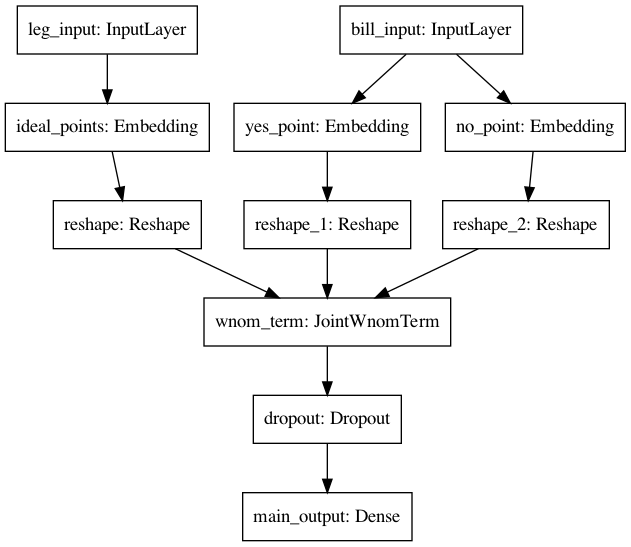
\includegraphics[width=0.75\linewidth]{model} 

}

\caption{\label{fig:model1}Base Model}\label{fig:unnamed-chunk-2}
\end{figure}

We rely on several simple techniques from machine learning 1. Out of
sample testing 2. Dropout regularization

Out of sample testing provides clear insight about the impact of a
decision. Does it make sense to add another dimension? How much do
dynamic ideal points help?

Dropout in two places: 1. Each dimension to ensure fitting even if first
dimensions dominates. 2. On bill embeddings (to not overfit to a
specific bill). Why not on legislators? The structure of the dynamic
part of the model doesn't allow this easily.

\section{Results}\label{results}

\subsection{My method and WNOMINATE packages are
similar}\label{my-method-and-wnominate-packages-are-similar}

\subsection{Let's do some things that weren't really feasible
before}\label{lets-do-some-things-that-werent-really-feasible-before}

\begin{enumerate}
\def\labelenumi{\arabic{enumi}.}
\tightlist
\item
  I implemented DW-NOMINATE as a neural network

  \begin{itemize}
  \tightlist
  \item
    Why? Because I could! But also because it's a nice platform for this
    kind of optimization.
  \item
    It scales much better than existing implementations
  \item
    It's extensible in very interesting ways
  \end{itemize}
\item
  All ideal point models are (a bit) overfit.

  \begin{itemize}
  \tightlist
  \item
    At some point the algorithm starts to make marginal improvements to
    the parameters that don't improve out of sample performance
  \item
    Out of sample performance matters much more than in sample (e.g.~if
    we only cared about in sample we'd just add dimensions until we cam
    predict it perfectly)
  \item
    Out of sample performance is a useful metric for evaluating modeling
    choices (adding another dimension, adding a time component, adding
    an external variable)
  \end{itemize}
\end{enumerate}

this is inline 42 and

\begin{Shaded}
\begin{Highlighting}[]
\NormalTok{py}\OperatorTok{$}\NormalTok{answer}
\end{Highlighting}
\end{Shaded}

\begin{verbatim}
## [1] "42"
\end{verbatim}

\begin{Shaded}
\begin{Highlighting}[]
\ControlFlowTok{pass}
\end{Highlighting}
\end{Shaded}

\begin{enumerate}
\def\labelenumi{\arabic{enumi}.}
\tightlist
\item
  How to implement in a neural network

  \begin{enumerate}
  \def\labelenumii{\alph{enumii}.}
  \tightlist
  \item
    Discuss both parameterizations
  \item
    Show convergence plots
  \item
    Discuss out of sample fit as the metrics of importance
  \end{enumerate}
\item
  A Neural Network implementation works

  \begin{enumerate}
  \def\labelenumii{\alph{enumii}.}
  \tightlist
  \item
    It estimates correctly on synthetic data (accuracy tables for both
    of these)
  \item
    It matches results from standard libraries (wnominate and pscl) on
    both synthetic and real data

    \begin{enumerate}
    \def\labelenumiii{\roman{enumiii}.}
    \tightlist
    \item
      Show both in sample and out of sample accuracy (will require
      writing a python wrapper to get predictions from the R results)
    \end{enumerate}
  \end{enumerate}
\item
  Results and applications of the neural network implementation

  \begin{enumerate}
  \def\labelenumii{\alph{enumii}.}
  \tightlist
  \item
    What are the optimal number of dimensions? Plot these and discuss
    tradeoffs
  \item
    Applying the model to cosponsorship
  \item
    Polarization differences

    \begin{enumerate}
    \def\labelenumiii{\roman{enumiii}.}
    \tightlist
    \item
      Votes models over time (how to do in multiple dimensions?)
    \item
      Compare between cosponsorship and votes
    \end{enumerate}
  \end{enumerate}
\end{enumerate}




\newpage
\singlespacing 
\end{document}
